Цель работы:
\begin{enumerate}
  \item исправить ошибки плагина TaskFirefoxWin;
  \item переделать программный модуль TaskThunderbirdWin в плагин для проекта coex.
\end{enumerate}

\subsubsection{TaskFirefoxWin}

Плагин TaskFirefoxWin предназначен для сбора истории посещений браузера Mozilla Firefox. История находится в файле базы данных places.sqlite, который расположен в C:\textbackslash Users\textbackslash User\textbackslash AppData\textbackslash Roaming\textbackslash Mozilla\textbackslash Firefox\textbackslash Profiles\textbackslash profilename.

Плагин выполняет рекурсивный обход директорий пока не найдет файл places.sqlite. Затем плагин подключается к базе данных, содержащейся в данном файле и выполняет sql-запрос на выборку данных из таблицы.
~\ref{teresh_1:teresh_1}

\begin{figure}[h!]
\center{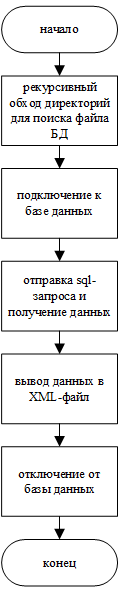
\includegraphics[width=0.2\linewidth]{teresh_1}}
\caption{ Блок-схема алгоритма TaskFirefoxWin }
\label{teresh_1:teresh_1}
\end{figure}

Программный модуль TaskFirefoxWin был некорректно переделан в плагин проекта coex. Вследствие чего, он не исполнялся. В результате тестирования было выявлено, что причиной некорректной работы плагина были служебные файлы TaskPlugin.pro, build.sh и taskFirefox.h. Были внесены исправления в эти служебные файлы. После этого плагин исполнялся.
~\ref{teresh_2:teresh_2}

\begin{figure}[h!]
\center{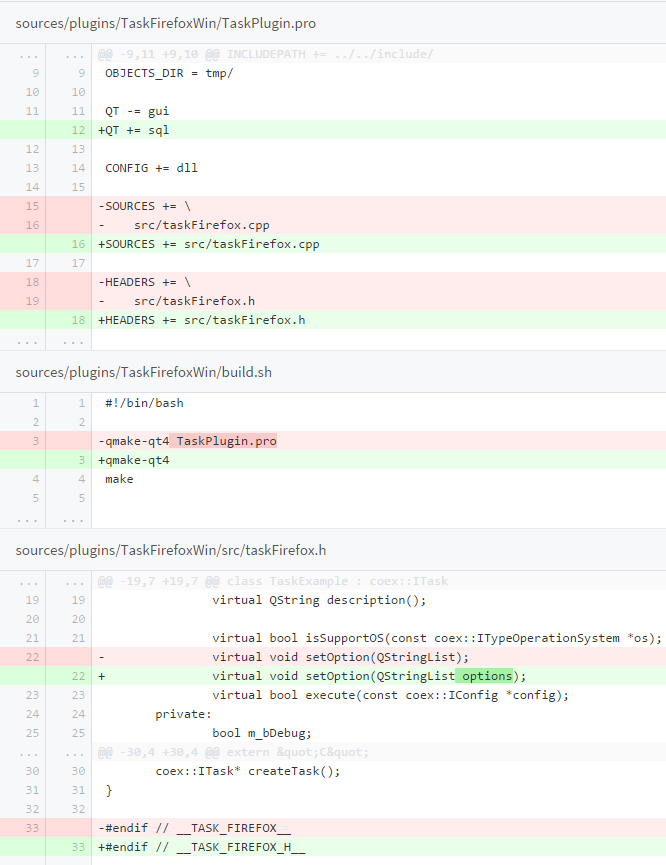
\includegraphics[width=0.6\linewidth]{teresh_2}}
\caption{ Изменения в служебных файлах }
\label{teresh_2:teresh_2}
\end{figure}

Были добавлены тестовые данные для проверки работоспособности плагина. Также был добавлен вывод результатов работы плагина в XML. В результате тестирования было выявлено, что плагин не выполняет поставленную задачу.

В одном из обновлений Mozilla Firefox была изменена структура файла places.sqlite. Из-за этого не работал sql-запрос для выборки данных из таблицы с историей посещений. Был составлен новый запрос: select * from moz\_places.
~\ref{teresh_3:teresh_3}

\begin{figure}[h!]
\center{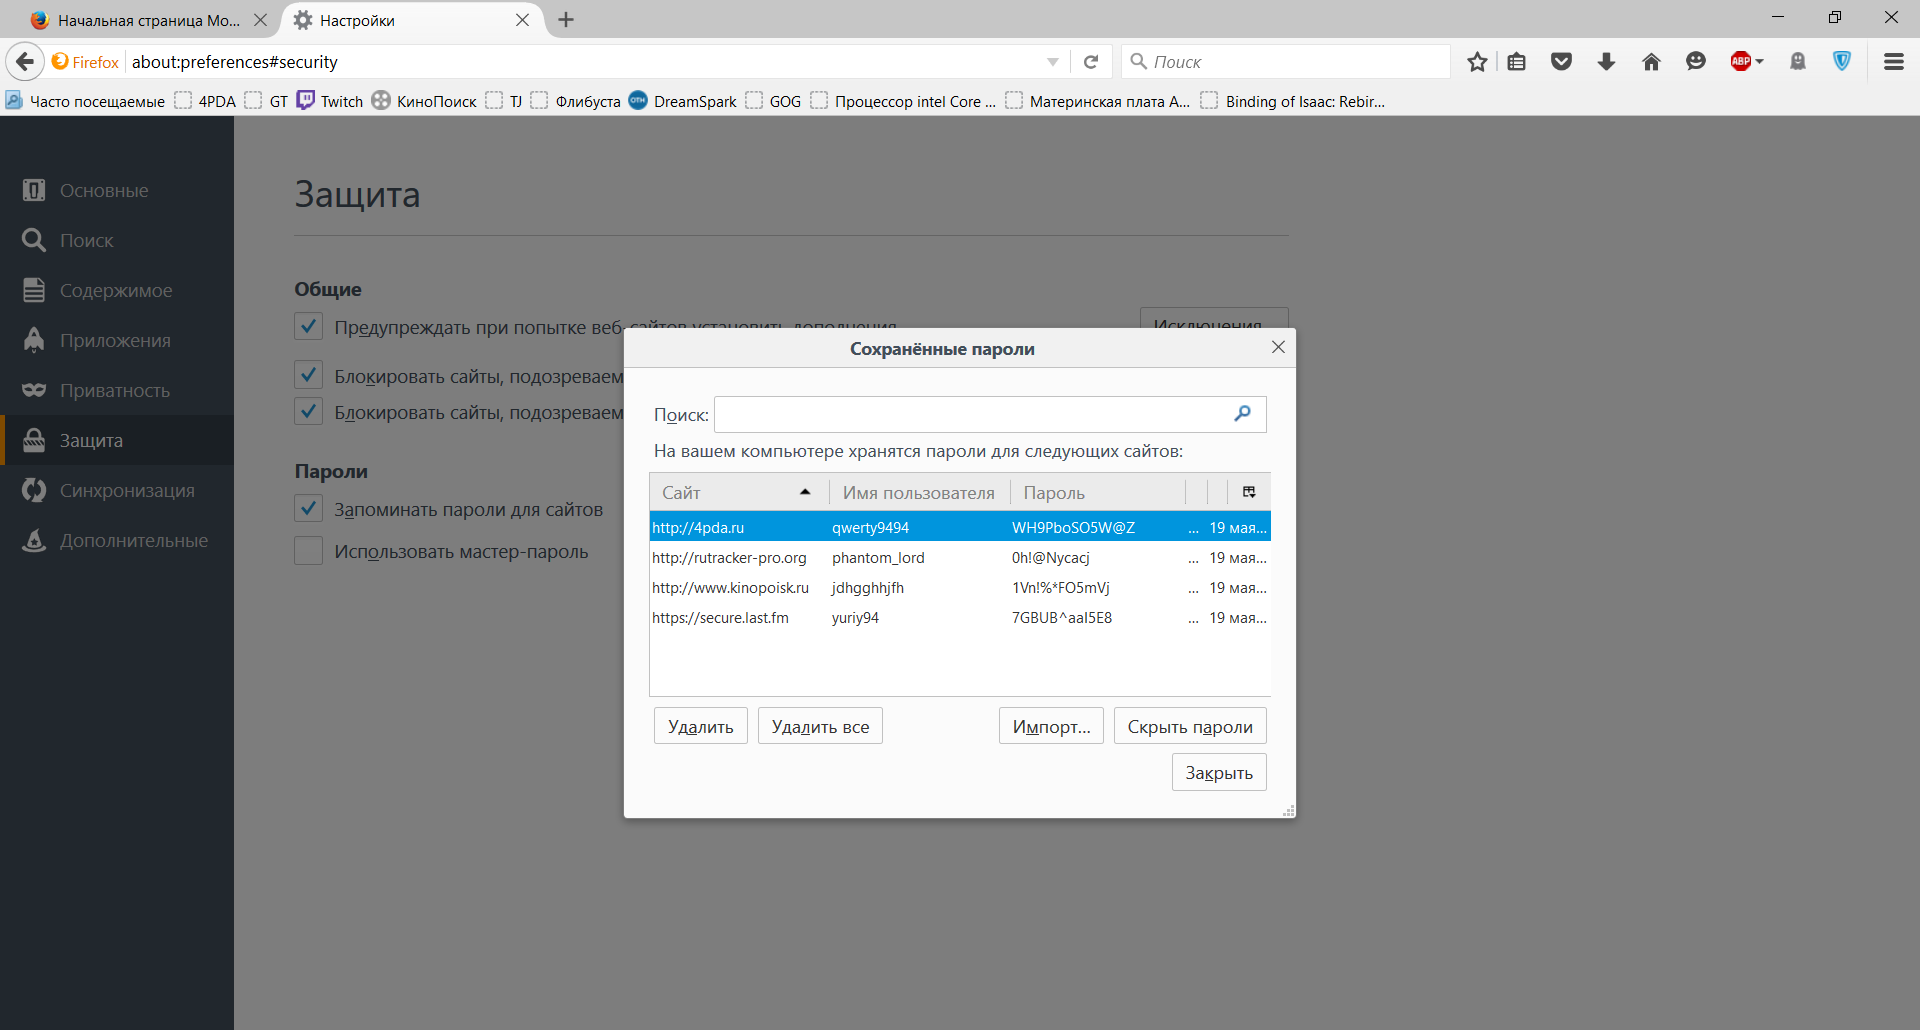
\includegraphics[width=0.7\linewidth]{teresh_3}}
\caption{ Структура базы данных и нужной таблицы }
\label{teresh_3:teresh_3}
\end{figure}

Было произведено тестирование исправленного плагина. Из представленных исходных данных был получен такой отчет в XML-файле.
~\ref{teresh_4:teresh_4}
~\ref{teresh_5:teresh_5} 

\begin{figure}[h!]
\center{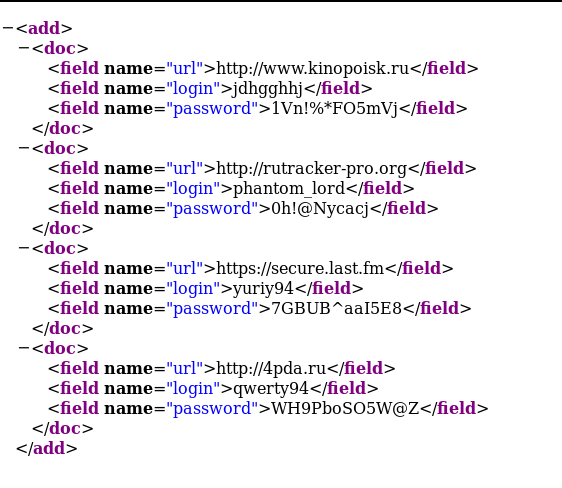
\includegraphics[width=0.5\linewidth]{teresh_4}}
\caption{ Тестовые данные }
\label{teresh_4:teresh_4}
\end{figure}

\begin{figure}[h!]
\center{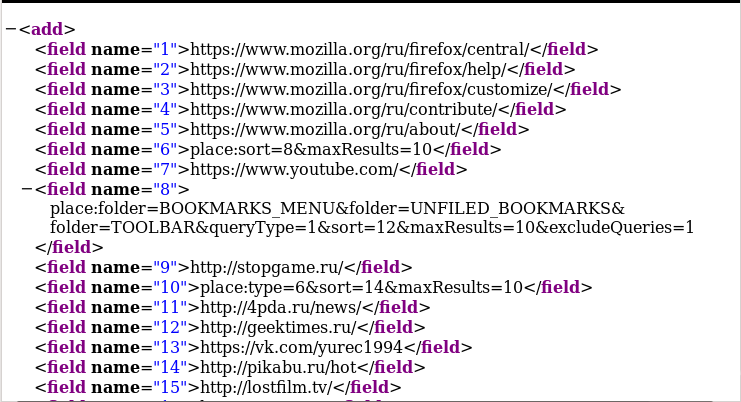
\includegraphics[width=0.6\linewidth]{teresh_5}}
\caption{ Результат тестирования TaskFirefoxWin }
\label{teresh_5:teresh_5}
\end{figure}

\subsubsection{TaskThunderbirdWin}

TaskThunderbirdWin был выполнен в виде отдельного программного модуля. Модуль предназначен для сбора сообщений и представления их в формате XML. Сообщения хранятся в файле Inbox.mbox для входящих сообщений и Sent.mbox для исходящих сообщений. Путь, по которому находятся файлы: C:\textbackslash Users\textbackslash User\textbackslash AppData\textbackslash Roaming\textbackslash Thunderbird\textbackslash Profiles\textbackslash profile\_name\textbackslash Mail\textbackslash server\_name. mbox представляет собой текстовый файл, в котором хранятся все сообщения почтового ящика. Начало почтового сообщения определяется строкой из 5 символов: словом <<From>> с последующим пробелом.

После открытия файл mbox разделяется на отдельные сообщения с помощью регулярного выражения <<(From \textbackslash \textbackslash r\textbackslash \textbackslash n)|(From \textbackslash \textbackslash n\textbackslash \textbackslash r)|From \textbackslash \textbackslash r|From \textbackslash \textbackslash n>>. Затем к каждому сообщению применяются регулярные выражения:

\begin{itemize}
  \item <<\textbackslash \textbackslash nDate: ([\textasciicircum \textbackslash \textbackslash n]*)\textbackslash \textbackslash n>> --- время отправки/приема сообщения;
  
  \item <<\textbackslash \textbackslash nFrom: .*([a-z][\textbackslash \textbackslash w\textbackslash \textbackslash .]*\textbackslash \textbackslash w@\textbackslash \textbackslash w[\textbackslash \textbackslash w\textbackslash \textbackslash .]*\textbackslash \textbackslash .\textbackslash \textbackslash w*).*\textbackslash \textbackslash nUser-Agent:>> --- кто отправил сообщения;
  
  \item <<\textbackslash \textbackslash nTo: .*([a-z][\textbackslash \textbackslash w\textbackslash \textbackslash .]*\textbackslash \textbackslash w@\textbackslash \textbackslash w[\textbackslash \textbackslash w\textbackslash \textbackslash .]*\textbackslash \textbackslash .\textbackslash \textbackslash w*).*\textbackslash \textbackslash nSubject:>> --- кто получил сообщение;
  
  \item <<\textbackslash \textbackslash nContent-Transfer-Encoding: 8bit\textbackslash \textbackslash s*(\textbackslash \textbackslash S.*\textbackslash \textbackslash S)\textbackslash \textbackslash s*[0-3]\textbackslash \textbackslash d\textbackslash \textbackslash .[01]\textbackslash \textbackslash d\textbackslash \textbackslash .\textbackslash \textbackslash d{4} [0-2]\textbackslash \textbackslash d:[0-5]\textbackslash \textbackslash d, [\textasciicircum \textbackslash \textbackslash n]*\textbackslash \textbackslash n>> --- текст сообщения.
\end{itemize}

~\ref{teresh_6:teresh_6}

\begin{figure}[h!]
\center{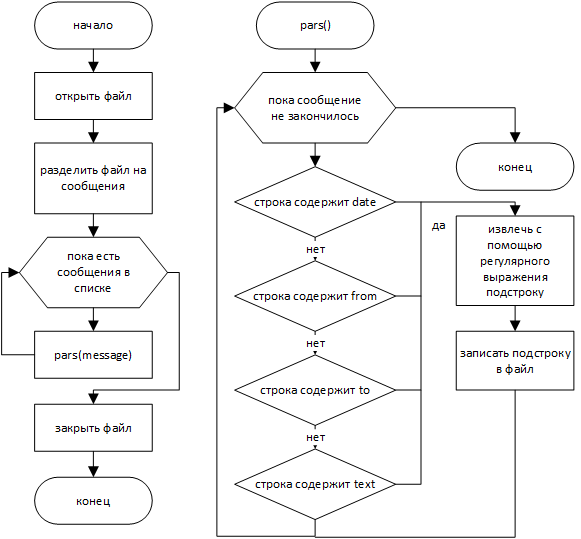
\includegraphics[width=0.6\linewidth]{teresh_6}}
\caption{ Блок-схема алгоритма TaskThunderbirdWin }
\label{teresh_6:teresh_6}
\end{figure}

Как отдельный модуль, TaskThunderbirdWin выполнял поставленные перед ним задачи.
~\ref{teresh_7:teresh_7}

\begin{figure}[h!]
\center{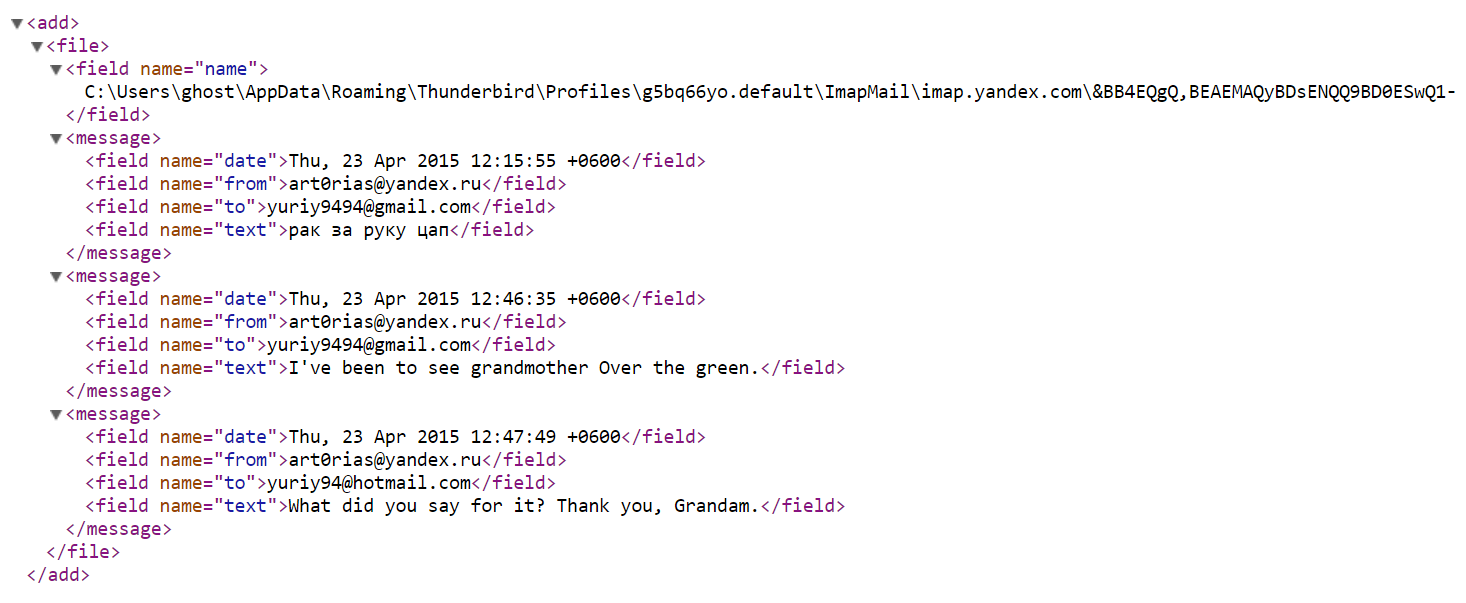
\includegraphics[width=0.9\linewidth]{teresh_7}}
\caption{ Результат тестирования TaskThunderbirdWin }
\label{teresh_7:teresh_7}
\end{figure}

Но после того, как TaskThunderbirdWin был переписан под архитектуру coex, возникли проблемы в работе данного модуля. Ведется тестирование с целью нахождения ошибок, мешающих корректному выполнению данного модуля.

\clearpage
